\begin{center}
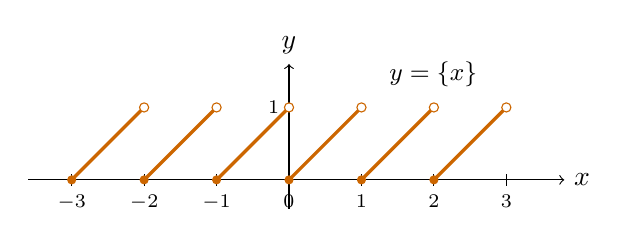
\begin{tikzpicture}[scale=0.92]
\draw[->] (-3.6,0)--(3.8,0) node[right]{$x$};
\draw[->] (0,-0.4)--(0,1.6) node[above]{$y$};
\foreach \n in {-3,-2,-1,0,1,2,3}{\draw (\n,0.08)--(\n,-0.08) node[below,font=\scriptsize]{$\n$};}
\draw (0,1) node[left,font=\scriptsize]{$1$};
\foreach \n in {-3,-2,-1,0,1,2}{
  \draw[orange!80!black,very thick] (\n,0)--(\n+1,1);
  \fill[orange!80!black] (\n,0) circle(1.8pt);
  \draw[orange!80!black,fill=white] (\n+1,1) circle(1.8pt);
}
\node[above right,font=\small] at (1.25,1.15) {$y=\{x\}$};
\end{tikzpicture}
\end{center}
